\documentclass[notitlepage,10pt,swedish,a4paper]{article}

\usepackage[utf8]{inputenc}
\usepackage[T1]{fontenc}

\usepackage{babel}

\usepackage{graphicx}
\DeclareGraphicsExtensions{.png,.jpg}

\begin{document}

\title{Furka OberAlpbahn och Steffenbach-bron}
\author{Stefan Skoglund}
\maketitle

1911 startade det franskfinansierade bolaget Compagnie suisse du Chemin de fer de la Furka (Brig-Furka-Ðisentis) bygget
av sin linje mellan staden Brig och via Andermatt i Gotthardpasset till staden Disentis i öst.

Med järnvägens 97 km långa linje förbinds de schweiziska kantonerna Wallis i övre delen av Rhône-dalen, Uri med sin flod Reuss (som via Luzernsjön är ett tillflöde till Rhen) med Disentis i kantonen Graubünden och dess flod Vorderrhein.

I Disentis finns en anslutning mellan meterspåriga Furka-Oberalp med likaledes meterspåriga Rhätische Bahn (RhB.)

Brig finns i den allra översta delen av Rhônedalen medans Andermatt är känt som entreporten från norr till Gotthardpasset.

Furka-passet är bergspassagen mellan Andermatt och Rhônedalen (Brig) medans Oberalp-passet är passagen över bergen till Disentis.
Alltså måste Furka-Oberalp passera två alppass vilket medförde bekymmer.

1914 var byggnation mellan Brig och Gletsch på Andermatt-sidan klar och trafik dit startades slutligen 1915.

Kriget medförde att kapitalflödet till banan från de franska investerarna sinade och eftersom banan inte var klar till Andermatt så var trafikinkomsterna otillräckliga. Bolaget tvånglikviderades via domstol 1923.
1925 förvärvade de närliggande järnvägsbolagen och kantonerna banan för 1750000 schweizerfranc och därefter bildades bolaget Furka-Oberalp-Bahn (FO). Via federala beslut i Bern finansierades byggnationen med 3.35 miljoner franc.
1926 öppnades linjen Brig-Andermatt-Disentis för genomgående trafik.
I samband med andra världskriget finansierades en elektrifiering av hela järnvägen och att Oberalp-sträckan skulle vintersäkras. Fram tills dess stängdes järnvägen vintertid pga svårigheterna att hålla den öppen.

1972 började byggnadsarbetena på den framtida Furka-Basistunnelen, en ny betydligt lägre placerad tunnel.

11 Oktober 1981 kördes sista kuggstångsförsedda tåget över Furka passet innan vinterstängningen.

26 Juni 1982 öppnade bolaget de två nya tunnlarna, en 673 m lång linjeomdragningstunnel och den 15442 långa Furka-Basistunnelen i och med detta kunde linjen Brig-Andermatt trafikeras med normala meterspåriga järnvägsfordon.

2003 gick namnet Furka-OberalpBahn tillsammans med Zermattbahn i graven i och med fusionen mellan dem och bildandet av Matterhorn-Gotthard-Bahn (MGB). En sammanhängande linje mellan orterna Zermatt vid Matterhorn till Disentis.

Furka-OberalpBahn och Rhätische Bahn är välkända utomlands för Glacierexpressen.

\section{Dampfbahn Furka-Bergstrecke}

Järnvägslinjen upp över passet skulle efter öppnandet av Basistunnelen rivas men en stor grupp av järnvägsvänner lyckades förhindra detta.

Från 1983 började arbetet att reparera och återställa den gamla järnvägslinjen över passet mellan Oberwald i Rhônedalen och Realp i öst och annonserad passagerartrafik mellan Realp och Tieffenbach återstartade 1992.
2010 återöppnades linjen (den på kartan svagt heldragna linjen) i hela sin sträckning.

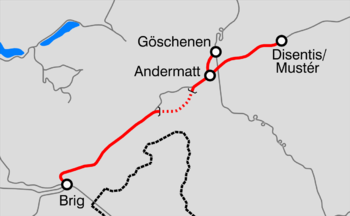
\includegraphics[width=150pt]{350px-FO_Bahnnetz}

\section{Steffenbach-brücke}
\label{sec:steffenbachbrucke}

Lavinfaran på Furka-delen demonstrerades mycket tydligt Maj 1916 när en lavin förstörde den vid ursprungliga byggnationen
över en fors på en höjd av 1765 möh i sten byggda järnvägbron.

Bron nybyggdes i stål 1925 av brobyggnadsfirman Theodor Bell \& Cie i en ovanlig konstruktion.

Järnvägen passerar bron med en stigning på 110 promille (den är försedd med kuggstång enligt Abt-systemet.)

Fackverket viks efter att kontaktledningen är nedmonterad med hjälp av handvevade vinschar ihop i två separata paket på hösten och dras därefter in i skydd på var sitt brohuvud.

Varje halva bär sin andel av den mellersta ca 13 meter långa brosektionen och stöds i sin tur av en panelsektion som med en rörlig led vilar mot stenfundament långt nedanför.

Ihopvikningen går till så att mittsektionen med hjälp av en hjälpbock på den västra sidan (se teckningen nedan, väster är till vänster) ned till lodrät läge. Därefter kan brosektionen på den östra sidan lyftas upp från sin vilopunkt på brofundamentet och sedan på järnvägstrallor dras in på järnvägsspåret. Pendelstödet följer då med och lägger sig mot brofundamentet och mittsektionen ligger i hela sin längd på pendelstödet.

Den västra sidans brosektion lyfts på samma sätt upp från sin vilpunkt , dras in på järnvägsspåret och tar samtidigt med sig sitt pendelstöd.

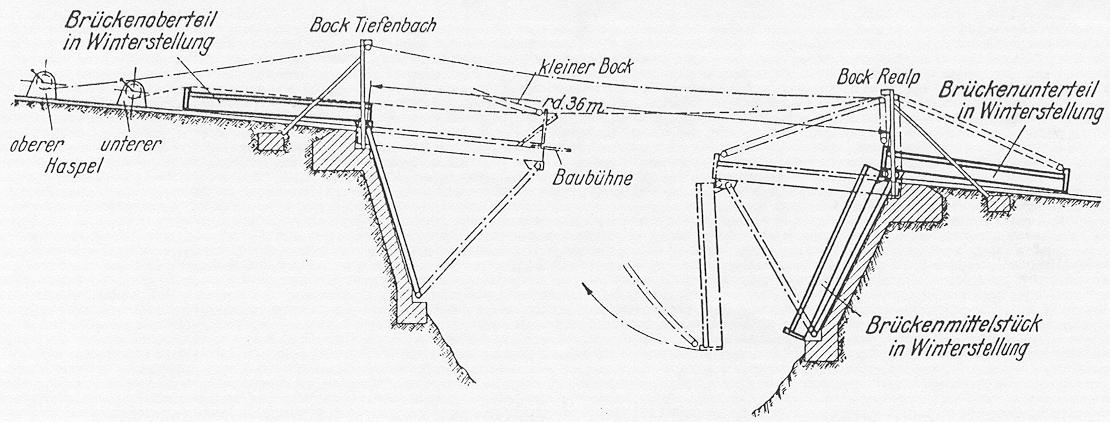
\includegraphics[width=300pt]{abb13_300}

Dagens museijärnväg har återställt bron i det här skicket.

\end{document}
